\documentclass{beamer}
\usepackage{graphicx}
\usepackage{multicol}
\usepackage{subfig}
\definecolor{Dgreen}{HTML}{1b5e20}
\definecolor{Mgreen}{HTML}{2e7d32}
\definecolor{Lgreen}{HTML}{388e3c}
\mode<presentation>
\usetheme{Madrid}
\setbeamercolor{palette primary}{bg=Dgreen,fg =white}
\setbeamercolor{palette secondary}{bg=Mgreen,fg=white}
\setbeamercolor{palette tertiary}{bg=Mgreen,fg=white}
\setbeamercolor{palette quaternary}{bg=Mgreen,fg=white}
\setbeamercolor{structure}{fg=Lgreen} % itemize, enumerate, etc
\setbeamercolor{section in toc}{fg=Mgreen} % TOC sections
\usepackage[export]{adjustbox}

\setbeamersize{text margin left=3mm,text margin right=5mm }
\geometry{paperwidth=420pt, paperheight=300pt}
\usepackage{verbatim}
\usepackage{tikz}
\usetikzlibrary{positioning}
\usepackage{tikz}
\usepackage{blindtext}
\graphicspath{{Images/}}
\setbeamercolor*{title}{use=structure,fg=white,bg=structure.fg}
\setbeamertemplate{title page}[default][colsep=-4bp,rounded=true,shadow=true]
\title{Tokamak 3D Equilibrium Reconstruction}
\subtitle{A Deep Learning approach}
\author{Lorenzo Rossi}
\institute{Università di Rome "Tor Vergata"} % chktex 18
\begin{document}
\begin{frame}
	\titlepage{}
	\vspace{-1cm}
	\begin{figure}
		\centering
		
\includegraphics[scale=0.3]{2022-06-06-23-17-53.png}% chktex 8
	\end{figure}
\end{frame}
\begin{frame}
	\frametitle{Contents}
	\tableofcontents
\end{frame}
\begin{frame}
	\frametitle{Introduzione}
	\section{Introduzione}
	L'obiettivo di questa tesina è quello di fornire una ricostruzione 3D del plasma in forma analitica.
	Tramite le equazioni MHD (\emph{MagnetoHydroDynamics}) è possibile considerare il plasma come un fluido conduttore soggetto all'azione di un campo magnetico.
	\begin{block}{Equilibrio}
		L'equilibrio è quella situazione in cui tutte le forze agenti su di essa hanno risultante nulla.
	\end{block}
	La ricostruzione dell'equilibrio del plasma è necessaria al miglioramento dell'efficienza fusionistica e alla protezione delle componenti che costituiscono il Tokamak.
\end{frame}
\begin{comment}
	\begin{frame}
	\frametitle{Dinamica del plasma}
	\section{Dinamica del plasma}
	La dinamica del plasma viene descritta da:
	\begin{itemize}
		\item Continuity equation (1):\(\frac{\partial\rho}{\partial t}+\nabla\cdot(\rho \nu)=0\);
		\item Momentum equation (3):\(\rho \frac{\partial\nu}{\partial t}+\rho(\nu\cdot\nabla)\nu=J\times B-\nabla p\);
		\item Ideal Ohm's law (3):\(E+\nu\times B=0\);
		\item Faraday's law (3):\(\frac{\partial B}{\partial t}=-\nabla\times E\);% chktex 18
		\item ``Low frequency'' Ampere's law (3):\(\mu_{0}J=\nabla\times B\);% chtex 18
		\item Magnetic divergence (1):\(\nabla\cdot B=0\);
		\item Energy (1):\(\frac{d}{dt}(\frac{p}{\rho^{\gamma}})\);
	\end{itemize}
\end{frame}
\end{comment}
\begin{frame}
	\frametitle{Equilibrio del plasma}
	\section{Equilibrio del plasma}
	Assumendo che:
	\begin{itemize}
		\item Il plasma si trovi in regime stazionario:\( \frac{\partial}{\partial t}=0\)
		\item Riferimento in v (\(\nu=0\));
	\end{itemize}
	Si ottiene:
	\begin{itemize}
		\item \(J\times B=\nabla p\)
		\item \(\mu_{0}J=\nabla\times B\)
		\item \(\nabla\cdot B=0\)
	\end{itemize}
\footnote{
	Dato \(f(x,y,z)=f_{1}\overrightarrow{i}+f_{2}\overrightarrow{j}+f_{3}\overrightarrow{k}\) si definiscono:
	\begin{itemize}
		\item Gradiente  \(\nabla f = \frac{\partial f}{\partial x}\overrightarrow{i}+\frac{\partial f}{\partial x}\overrightarrow{j}+\frac{\partial f}{\partial x}\overrightarrow{k} \);
		\item Divergenza \(\nabla\cdot f=\frac{\partial f_{1}}{\partial x}+\frac{\partial f_{2}}{\partial y}+\frac{\partial f_{3}}{\partial z}\);
		\item Rotore \(\nabla\times f=\left\lvert \begin{matrix}
			\overrightarrow{i}&\overrightarrow{k}&\overrightarrow{k}\\
			\frac{\partial}{\partial x}& \frac{\partial}{\partial y}&\frac{\partial}{\partial z}\\
			f_{1}&f_{2}&f_{3}
		\end{matrix}\right\rvert \)
	\end{itemize}
}
\end{frame}
\begin{frame}
	\frametitle{Grad-Shafranov}
	\section{Grad-Shafranov}
	\begin{minipage}[t]{0.50\textwidth}
		Per giungere infine all'equazione di Grad-Shafranov occorre supporre simmetria toroidale. In particolare:
		\begin{equation*}
			\frac{\partial}{\partial \phi}=0
		\end{equation*}

	\end{minipage}
	\begin{minipage}[t]{0.40\textwidth}
		\begin{figure}
			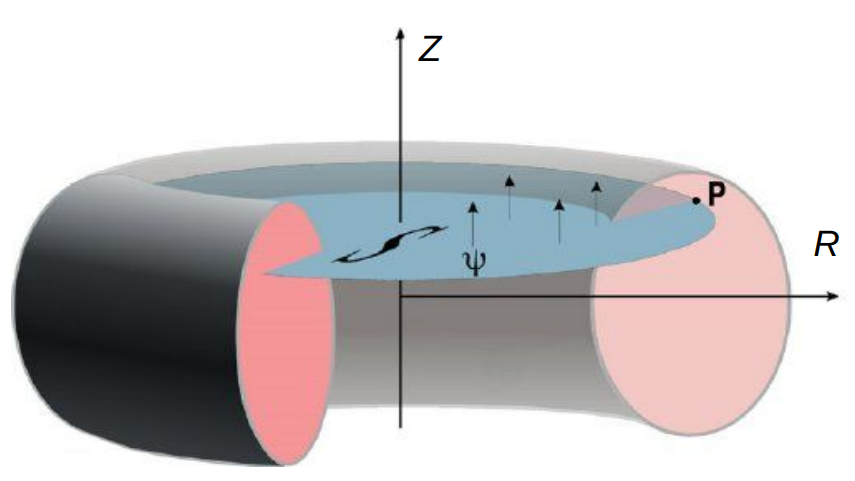
\includegraphics[scale=0.25]{2022-06-07-13-08-40.png}% chktex 8
			\caption{Simmetria toroidale Tokamak}
		\end{figure}
	\end{minipage}
	\begin{block}{Equazione di Grad-Shafranov}
		\begin{align*}
			p                                                                                                                           & =f(\psi)                                                          \\
			F                                                                                                                           & =g(\psi)                                                          \\
			\frac{\partial^{2}\psi}{\partial r^{2}}-\frac{1}{r}\frac{\partial \psi}{\partial r}+\frac{\partial^{2}\psi}{\partial z^{2}} & =-\mu_{0}r^{2}\frac{d p}{d \psi}-\frac{1}{2}\frac{d F^{2}}{d\psi}
		\end{align*}
	\end{block}
\end{frame}
\begin{frame}
	\frametitle{Limitazioni}
	\begin{minipage}[t]{0.45\textwidth}
		\begin{figure}
			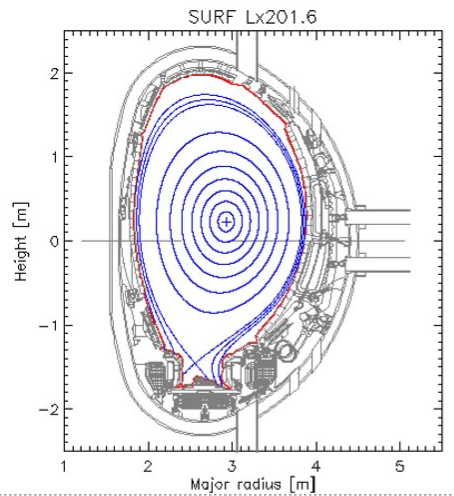
\includegraphics[scale=0.4]{2022-06-07-13-17-56.png}% chktex 8
		\end{figure}
	\end{minipage}
	\begin{minipage}[t]{0.45\textwidth}
		Sebbene questo metodo consenta di ricostruire efficientemente l'equilibrio del plasma. Tuttavia:\begin{itemize}
			\item Il plasma non è sempre in regime stazionario;
			\item La simmetria toroidale non è sempre rispettata.
		\end{itemize}
	\end{minipage}\\
	\medskip
	Una valida alternativa per ottenere più informazioni sul processo in questione viene fornita dal metodo Physics Informed Neural Network basati sul deep learning.
\end{frame}
\begin{frame}
	\frametitle{Deep Learning}
	\section{Deep Learning}
	\begin{block}{Deep Learning}
		Il deep Learning è una branca del Machine Learning che studia l'apprendimento automatico tramite l'utilizzo di architetture stratificate dette \textbf{neural  network multilayers}.
	\end{block}
	\begin{itemize}
		\item L'unità fondamentale di una neural network multilayers è il \textbf{neurone} che esegue una singola operazione non lineare.
		\item Ogni neurone viene connesso con uno o più neuroni in base all'organizzazione della rete;
		\item L'architettura più utilizzata è di una rete stratificata in feedforwar\begin{itemize}
			\item La connessione tra neuorni avviene solo tra livelli adiacenti
		\end{itemize}
		\item Utilizzo della \textbf{backpropagation}: i pesi associati ad ogni neurone vengono aggiornati calcolando l'uscita della rete e propagando l'errore all'indietro verso i livell più alti
	\end{itemize}
\end{frame}
\begin{frame}
	\frametitle{Physics Informed Neural Network}
	\section{Physics Informed Neural Network}
	\begin{block}{Physics Informed Neural Network}
		Il Physics Informed Neural Network è un metodo di deep learning basato su reti neurali per risolvere le PDE (\emph{Partial Differential Equation}).
	\end{block}
	\begin{itemize}
		\item Permettono di risolvere numericamente equazioni differenziali molto complesse;
		\item Le soluzioni delle PDE minimizzano una funzione di costo dipendente dalle equazioni fisiche;
		\item La funzione di costo deve essere ben modellata per aderire al modello preso in considerazione;
		\item Processo di training elevato;
		\item Si necessitano di condizioni al contorno;
	\end{itemize}
\end{frame}
\begin{frame}
	\frametitle{PDE Neural Network - Struttura} % chktex 8
	\section{PDE Neural Network}
	\subsection{Struttura}
	Per la rete neurale si è scelto di utilizzare:
	\begin{itemize}
		\item Rete \textbf{fullyconnect}: ogni neurone di ogni livello è collegato con i neuroni del livello successivo;
		\item Backpropagation tramite di errore;
		\item Ogni neurone applica l'input una tangentoide;
	\end{itemize}
	\begin{figure}
		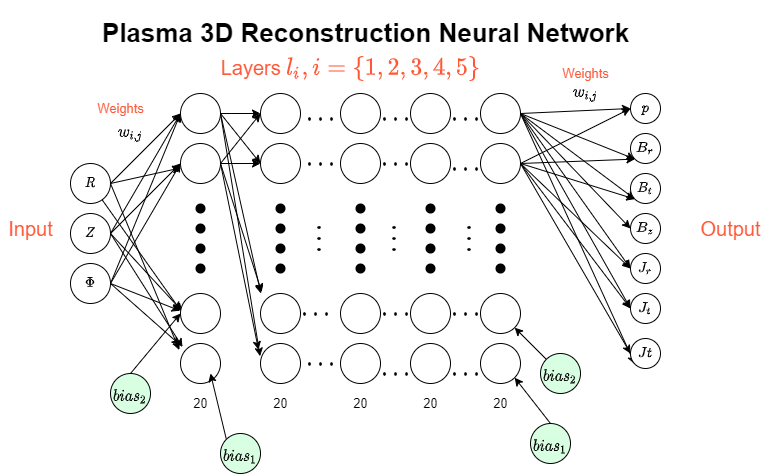
\includegraphics[scale=0.3]{reteOrganizzazione.png}
	\end{figure}

\end{frame}
\begin{frame}
	\frametitle{PDE Neural Network}
	\subsection{Errore}
	\vspace{-0.1cm}
		\begin{figure}
			\adjustimage{scale=0.37,left}{LossFunction.drawio.png}% chktex 8
		\end{figure}
\end{frame}
\begin{frame}
	\frametitle{Condizioni al contorno}
	\section{Condizioni al contorno}
	La soluzione delle PDE in \(\phi = \{ 0,2\pi \} \) potrebbe portare a soluzione diverse quando queste, per periodicità, devono essere identiche. Per evitare questo comportamento, occorre aggiungere una quinda funzione di costo:\begin{equation*}
		Loss5 = \frac{mean{(p-p_{f})}^{2}}{mean{(p_{f})}^{2}}+\frac{mean{(B_{r}-B_{r,f})}^{2}}{mean{(B_{r,f})}^{2}}+\frac{mean{(B_{z}-B_{z,f})}^{2}}{mean{(B_{z,f})}^{2}}+\frac{mean{(B_{t}-B_{t,f})}^{2}}{mean{(B_{t,f})}^{2}}
	\end{equation*}
	\begin{equation*}
		Loss6 = \frac{mean{(p-p_{i})}^{2}}{mean{(p_{i})}^{2}}+\frac{mean{(B_{r}-B_{r,i})}^{2}}{mean{(B_{r,i})}^{2}}+\frac{mean{(B_{z}-B_{z,i})}^{2}}{mean{(B_{z,i})}^{2}}+\frac{mean{(B_{t}-B_{t,i})}^{2}}{mean{(B_{t,i})}^{2}}
	\end{equation*}
\end{frame}
\begin{frame}
	\frametitle{Risultati}
	\section{Risultati}
		Risultato atteso:
		\begin{figure}
			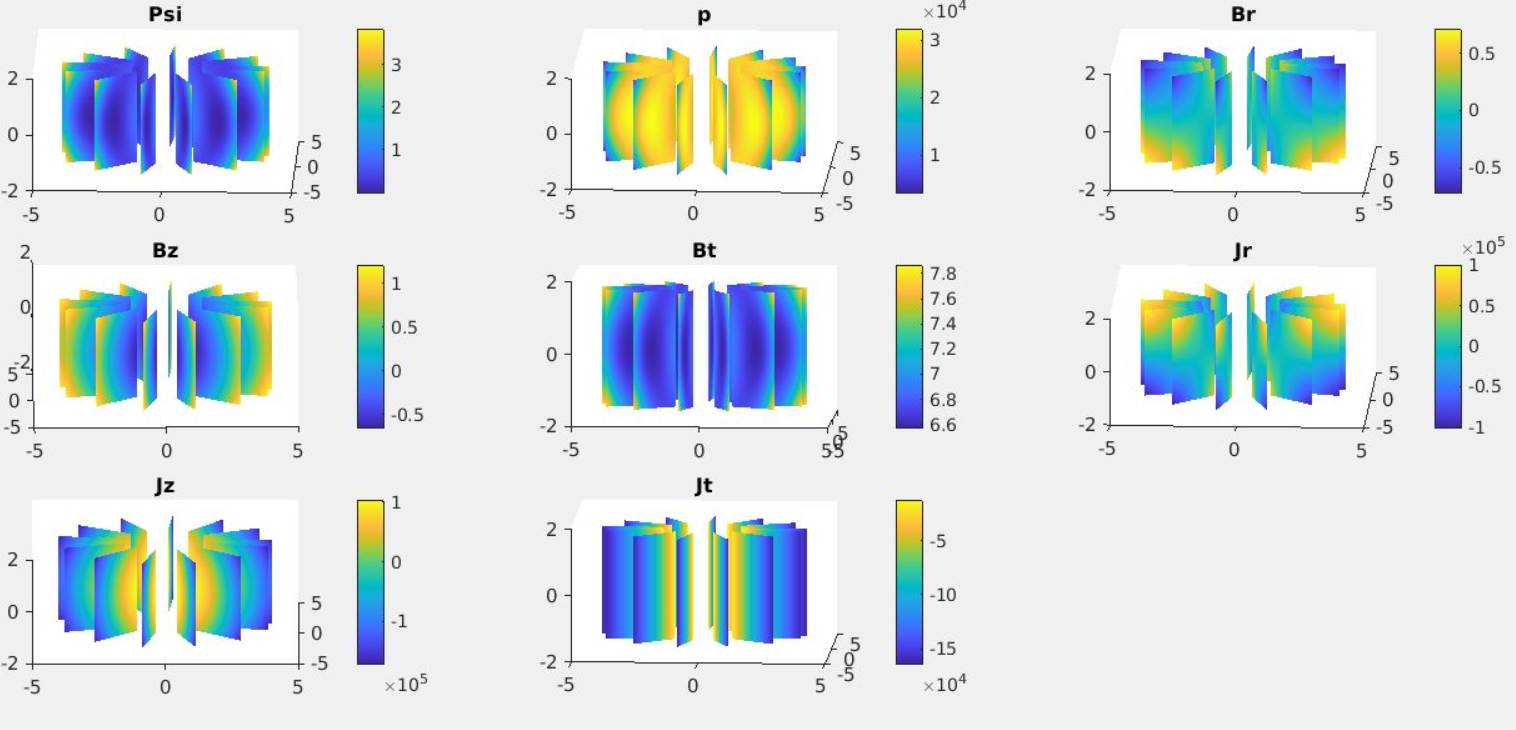
\includegraphics[scale=0.3]{2022-06-20-23-05-27.png}% chktex 8
		\end{figure}
\end{frame}
\begin{frame}
	\frametitle{Risultati}
	\begin{figure}
		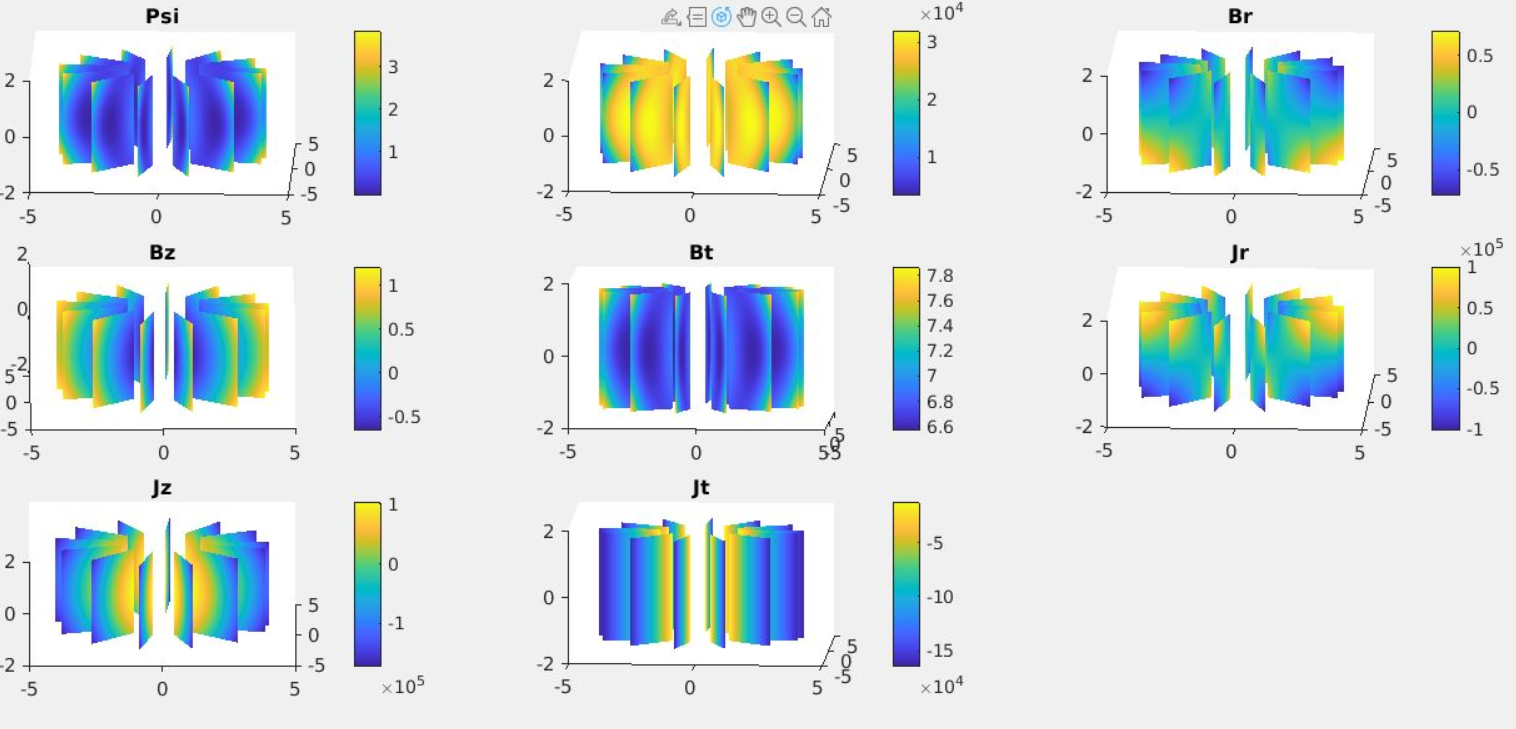
\includegraphics[scale=0.26]{2022-06-20-23-07-41.png}% chktex 8
		\caption{Risultato finale: 10000 epoche (16h di training)}% chktex 8
	\end{figure}
	\vspace{-1cm}
\footnote{\scriptsize
Learning eseguito su una macchina Dell XPS 8940:\\
		\begin{itemize}
			\item CPU Intel i7-11700 8c/16t @4.8Ghz;%chktex 8
			\item RAM:32GB DDR4;
			\item GPU:Nvidia RTX 3070;% chktex 29
			\item OS:Debian GNU Linux 10 \(\times \)86\_64;%chktex 8
		\end{itemize}
}
\end{frame}
\begin{frame}
	\frametitle{Considerazioni}
	\section{Considerazioni}
	\begin{itemize}
		\item Il risultato ottenuto è congruente alla configurazione reale;
		\item L'addestramento tramite GPU può abbattere notevolmente il tempo di addestramento;
		\item Le PDE utilizzate assumono che \(\frac{\partial}{\partial\phi }\neq 0\) e quindi la rete neurale potrebbe essere utilizzata anche per configurazioni asimmetriche;
		\item Una maggiore risoluzione di \(\phi \) può aumentare notevolmente la spesa computazionale.
	\end{itemize}
\end{frame}
\end{document}